\documentclass[11pt]{article}
\usepackage[margin=1in]{geometry}
\usepackage{xcolor}
\usepackage{amsmath,amssymb}
\usepackage{graphicx}
\usepackage{hyperref}
\usepackage{microtype}
\usepackage{enumitem}
\setlength{\emergencystretch}{3em}
\graphicspath{{../manuscript/figures/}}

\definecolor{revisionblue}{RGB}{0,70,180}
\newcommand{\Question}[1]{\par\medskip\noindent\textbf{Reviewer comment:}\par\begin{quote}\itshape #1\end{quote}}
\newcommand{\Answer}[1]{\par\noindent\color{black}\normalfont\textbf{Response:} #1\par\smallskip}
\newcommand{\Change}[1]{\par\noindent\color{revisionblue}\normalfont\textbf{Changes in the manuscript:} #1\par\color{black}\medskip}

\begin{document}

\begin{center}
{\Large Response to the Reviewers}\par
\vspace{0.4em}
{\large ``Special Optimal Thermal Cell: Correlator-Designed Supercells for Effective-Harmonic Phonons and Thermodynamics''}\par
\vspace{0.3em}
Albert Linda
\end{center}

We thank the reviewers for the detailed and technically constructive reports.
Each numbered comment is reproduced below. Our responses are in black,
and the corresponding manuscript revisions are summarized in blue. We have
substantially narrowed the claims, removed results that could not be validated,
added direct numerical controls, and made unresolved limitations explicit. A
final consistency audit also relabeled the experimental heat-capacity column as
calorimetric $C_p$ rather than $C_V$, withdrew the resulting like-for-like
accuracy claim, and corrected the Ag, Mo, and MgO experimental citations.

\section*{Revision at a glance}

To make the scope of the revision unambiguous, the principal new evidence can
be located as follows in the clean revised manuscript:
\begin{itemize}[leftmargin=1.5em]
\item \textbf{Matched displacement selection:} Fig.~3 (p.~9), with methods in
Secs.~III.A--B (pp.~4--5), interpretation and force-call accounting in
Secs.~V.A--B (pp.~11--12), and limitations in Sec.~V.D (p.~13).
\item \textbf{Polar non-analytic corrections and neutron data:} Figs.~4--5
(p.~10), including all three polar compounds and 39 tabulated NaCl neutron
points; scope is stated in Sec.~V.D (p.~13).
\item \textbf{IFC rank and predictive validation:} Table~III and Fig.~6
(p.~12), with the distinction between rank, regularization, predictive error,
and iteration count in Secs.~V.A--B and Appendix~E.
\item \textbf{MSD convention and residual forces:} Secs.~III.A and IV.E
(pp.~4 and 9) and Appendices~D (p.~15) and H (p.~17).
\item \textbf{Reproducibility:} exact electronic inputs, scripts, seeds, file
formats, and validation paths are listed in Appendix~J (p.~18).
\end{itemize}

The revised claim is deliberately narrower than the submitted one. We do not
claim a universal SOTC accuracy or speed advantage, a variational free-energy
bound, converged QHA, transport properties, or full outer-loop superiority.
The supported result is a reproducible effective-FC2 displacement-design
workflow whose sampling accuracy is comparable to the canonical median for the
nominal initialization in the three matched tests and whose operational
sensitivity to the coupled trial-model/optimizer initialization is now measured
explicitly.

\section*{Reviewer 1}

\Question{1. A major revision of the introduction, in particular when it comes to the mentions of TDEP and the sSCHA, is mandatory. For example, the author writes that \textquotedblleft{}The Temperature-Dependent Effective Potential (TDEP) approach [5, 6] generates displacements from a stochastic distribution matching the harmonic Bose--Einstein statistics of a trial phonon model''. This is not what TDEP is. TDEP is an interatomic force constant fitting method, and has nothing to do with sampling. It instead takes the displacements and forces from a sampled canonical ensemble and fits IFCs via least-squares. In fact, the most common usage of TDEP is to sample from molecular dynamics and fit from that data. The author is clearly mistaking stochastic sampling for TDEP. The definition of the sSCHA should also be revised, as it arises as a method for force fitting (which the SCHA indeed is) but then sticks to mentioning the sSCHA (sampling + force fitting). Furthermore, the mention of compact TDEP is puzzling, as that is at least to my knowledge not common terminology for any variation of TDEP and the work cited as a reference corresponds to the seminal paper for sTDEP. This mention should also be heavily revised. Finally, the claim that \textquotedblleft{}TDEP uses many random displacement configurations to statistically sample the thermal distribution'' is incorrect even if we ignore the misunderstanding on the definition of TDEP. Even if we just consider sTDEP, the configurations used to fit the force constants are not random, but distributed according to a Gaussian probability density function. The claim that \textquotedblleft{}It differs from SSCHA in that no variational minimization of a free-energy functional is required'' is also incorrect. They are inherently different methods to fit force constants. Furthermore, if we compare only sTDEP and sSCHA, they actually reduce to the same level of theory and reach the same results even from the free energy perspective, with the methodology with which it is minimized being the only real difference. In section V.c) the author again claims \textquotedblleft{}TDEP [5, 6] and SSCHA [7, 8] both rely on large ensembles of stochastically displaced supercells and converge IFCs or variational density matrices by statistical averaging.'' Again, this is untrue, stochastic sampling is one option of many.

I suggest the author familiarizes themselves with the following in order to properly edit this section: 10.1088/1361-648X/ac066b, \url{https://doi.org/10.1103/PhysRevB.96.014111}, \url{https://doi.org/10.1103/PhysRevB.87.104111}, \url{https://doi.org/10.1103/PhysRevB.95.014302}, \url{https://doi.org/10.1103/PhysRevB.89.064302}, \url{https://doi.org/10.1063/5.0174255}, \url{https://doi.org/10.1103/PhysRevB.84.180301}, \url{https://doi.org/10.1103/PhysRevB.88.144301}.}

\Answer{We agree. The earlier text conflated an IFC-fitting framework with one
possible source of displacement--force data. The revision defines TDEP as IFC
fitting, SCHA as the variational effective-harmonic level, and SSCHA as a
stochastic sampling and optimization implementation. It now also acknowledges
the reviewer's central equivalence point: with consistent ensembles, estimators,
and converged sampling, stochastic TDEP and SSCHA can reach the same
effective-harmonic stationary solution and free energy, although their numerical
minimization procedures differ. The nonstandard term ``compact TDEP'' and all
claims that TDEP intrinsically uses random configurations were removed.}

\Change{The Introduction and Sec.~V.C now define TDEP, SCHA, and SSCHA
separately, state the converged effective-harmonic sTDEP--SSCHA equivalence, and
require matched observables for cost/accuracy comparisons. Appendix~G states
that finite moment matching and ridge fitting do not inherit a
Gibbs--Bogoliubov upper bound. Blanket superiority claims over TDEP, SSCHA, and
AIMD were deleted. All eight works recommended in the comment are now cited in
the revised discussion (Refs.~5--8, 10, and 50--52). These changes appear in
the Introduction (p.~1), Sec.~V.C (p.~13), and Appendix~G (p.~17).}

\Question{2. Comparisons with Phonopy and TDEP are shown in almost every figure, but no parameters for these calculations are ever shown. This is a very big problem, as it effectively renders any comparisons impossible. What code was used? What q-point grids? What sampling? How many configurations? What cutoffs? These need to be included in order to substantiate any comparative claims with respect to these approaches. The computational cost claims are also unverifiable without such details, and so that point of the manuscript is so far unproven.}

\Answer{We agree that the old comparisons were not auditable. Every
undocumented TDEP curve and universal external-method speedup claim was removed.
We replaced them with a fully archived, like-for-like displacement-selection
test using Quantum ESPRESSO~7.5, PBE, the same equilibrium structures and
pseudopotentials, and the same $3\times3\times3$ primitive-cell supercells:
27 atoms for Al at 300~K, 27 for W at 1500~K, and 54 for NaCl at 700~K.
Wave-function/charge-density cutoffs and supercell $k$ meshes are
40/320~Ry and $4\times4\times4$ for Al, 30/240~Ry and
$4\times4\times4$ for W, and 60/480~Ry and $2\times2\times2$ for NaCl.
All calculations use a $10^{-9}$~Ry SCF threshold; the metals use 0.02~Ry
Marzari--Vanderbilt smearing and NaCl uses fixed occupations.

The conventional references were generated by central finite displacements
with Phonopy~2.9.1 (two displaced states for Al and W and four for NaCl).
Every sampled model uses reference-force subtraction, translational-drift
projection, ridge coefficient $10^{-3}$, central-force projection, the acoustic
sum rule, and FC2 cutoffs 4.5, 5.0, and 4.3~\AA. Dispersions are compared by
sorting branches pointwise on the same 251-point paths:
$\Gamma$--X--W--K--$\Gamma$--L for Al and NaCl and
$\Gamma$--H--N--$\Gamma$--P--H for W. The unchanged 20-snapshot test set is
used only for force prediction.

At $N=1,2,4,8,16$ displaced-force calls, 20 seeded permutations of the same
80-snapshot canonical-Gaussian training pool are compared with three
pre-specified, independently optimized correlator-matched sequences initialized
at $0.75T_D$, $T_D$, and $1.25T_D$. Their 48 new QE states per material all
completed with finite forces. For transparency, the canonical-pool median
displacement RMS values are 0.0870, 0.0872, and 0.2031~\AA, while the
nominal-$T_D$ design values are 0.0899, 0.0978, and 0.1701~\AA for Al, W, and
NaCl; no post hoc amplitude rescaling was applied.

At 16 calls, the pre-specified nominal-$T_D$ dispersion RMSEs are
0.425, 0.223, and 0.548~THz, compared with canonical medians
0.412, 0.207, and 0.564~THz. Thus nominal SOTC is 3.2\% and 8.1\% worse for
Al and W and 2.8\% better for NaCl: it is comparable, not uniformly superior.
The three-initialization ranges are 0.404--0.574, 0.178--0.377, and
0.459--0.928~THz. Nominal held-out-force errors
(0.104, 0.282, and 0.333~eV~\AA$^{-1}$) are likewise essentially the
canonical medians (0.104, 0.281, and 0.332~eV~\AA$^{-1}$). We report all
pre-specified sequences rather than selecting only the favorable one. The
comparison tests first-stage displacement selection; it is not presented as a
normalized wall-time speedup or a full self-consistent outer-loop comparison.}

\Change{The complete protocol is given in Secs.~III.A--B (pp.~4--5) and
Appendix~J (p.~18); Fig.~3 (p.~9) reports every force-call count, all 20
canonical seeds, all three initialization sequences, and both dispersion and
held-out-force errors. Sections~V.A--B (pp.~11--12) and V.D (p.~13) state the
initialization dependence and withdraw universal advantage and wall-time
speedup claims.}

\begin{figure}[htbp]
\centering
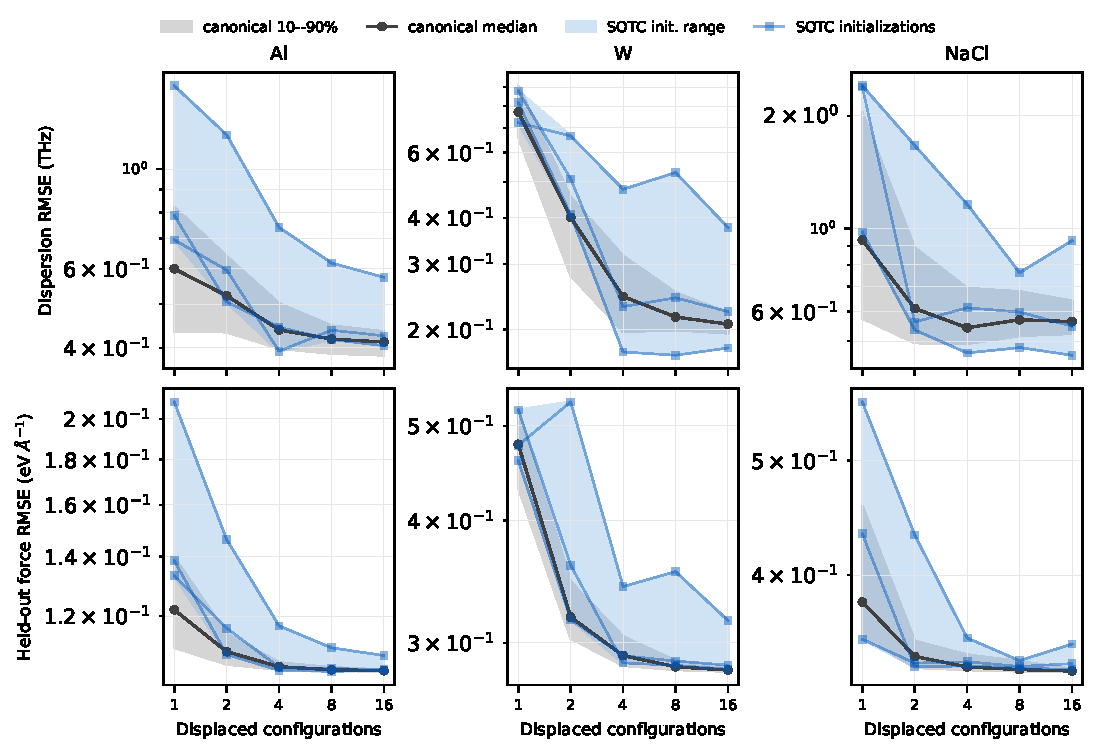
\includegraphics[width=\textwidth]{fig_matched_sampling.pdf}
\caption{Matched displacement-selection control used for the revised sampling
claim. Dispersion RMSE (left) and held-out force RMSE (right) are plotted
against 1, 2, 4, 8, and 16 displaced-force calls. Black bands show the
10--90\% range over 20 canonical seeds; colored curves show all three
pre-specified correlator-matched sequences. Cells, electronic settings, force
processing, fitting choices, held-out data, q paths, and force-call counts are
identical.}
\end{figure}

\Question{3. The mean square displacements differ by a factor of 2 or more for some of the systems computed but this fact is completely brushed off and is left entirely undiscussed in the manuscript. This is the largest discrepancy compared to experiment reported in the paper. The author must address this discrepancy.}

\Answer{The reviewer correctly identified a factor-of-three convention error. We now use the crystallographic one-component parameter $U_{\rm iso}=\langle|\mathbf u|^2\rangle/3$ everywhere and $B=8\pi^2U_{\rm iso}$. Reinterpreting the archived total three-dimensional MSD fields at 300~K gives $U_{\rm iso}=0.01088$, 0.00605, and 0.00516~\AA$^2$ for Al, Au, and Cu. Al is within the cited 0.010--0.011~\AA$^2$ interval. Au is 53--64\% low and Cu is 36--48\% low. We therefore do not claim general Debye--Waller agreement; the unstable Au spectrum is excluded from physical interpretation, and the Cu discrepancy is retained as a limitation.}

\Change{Equations~(3) and (12), Sec.~IV.E, Appendix~H, the code path, and analytic Einstein tests now use the same $U_{\rm iso}$ convention. Section~IV.E reports the corrected values, experimental ranges, and percentage discrepancies explicitly.}

\Question{4. Figure 6c) disagrees with table 3 and shows no agreement between QHA and the Gruneisen method. Furthermore, the explanation for the discrepancy at 300K is that it \textquotedblleft{}reflects a numerical artifact in the QHA finite-difference derivative near the inflection of V(T) at low temperature''. However, in the same table at 100K the value is reported to be in close agreement, which calls into question the proposed source of error. A proper investigation and fix for this error, and revision of the discrepancy between figure 6c) and table III is required.}

\Answer{We agree. The available three-volume data do not support a defensible QHA derivative or the previously quoted 300~K expansion coefficient. Rather than retain an underconverged result, we removed the QHA calculation, Figure~6, its table, the anomalous number, and all dependent accuracy claims. The revised manuscript is a fixed-volume effective-FC2 study.}

\Change{The abstract, theory, computational details, Results, Discussion, appendices, and Conclusions no longer contain a QHA result, QHA accuracy claim, or the anomalous expansion value. The phrase ``quasi-harmonic'' remains only where the manuscript explicitly states that quasi-harmonic theory lies outside the demonstrated scope.}

\Question{5. The approach to the free energy minimization raises some concerns. The number of volumes being used is remarkably low, and the method by which the expanded volume IFCs are obtained might work in these specific cases, but that is left to chance unless compared with the normally obtained ones and relies on very well behaved IFCs. Birch-Murnaghan is also 3rd order at minimum, not a parabola, so the fit can very likely be underdetermined. The justification for a parabolic fit needs proving especially when systems such a PbTe, which is extremely sensitive to parameterization, are under study. Furthermore, using E0 from DFT makes it so the free energy is not variational anymore, which calls the entire methodology into question without more complete validation.}

\Answer{We agree that the archived data cannot establish a converged equation of state, an expanded-volume IFC extrapolation, a controlled volume derivative, or a variational QHA bound. The entire QHA extension was therefore removed rather than defended. No parabolic fit is called Birch--Murnaghan; no volume-extrapolated IFC, thermal expansion, $C_P$, or QHA variational statement remains. PbTe is discussed only at fixed volume and is not used to validate thermal expansion. Appendix~G now makes the narrower variational statement explicit: matching a finite set of moments and performing ridge force fitting does not minimize the Gibbs--Bogoliubov functional and is not assigned a rigorous upper bound.}

\Change{All former QHA equations, equation-of-state fits, volume interpolation/extrapolation, free-energy minimization, figures, tables, and appendices were deleted. Sections~V.D and VI state that thermal expansion and $C_P$ require static energies and phonons over a converged volume grid and lie outside the demonstrated scope. The remaining thermodynamic scope is fixed-volume $C_V$, ZPE, $F_{\rm vib}$, and $S_{\rm vib}$.}

\Question{6. There are many cases of latex mistakes in the manuscript. A few examples can be found in pages 11, 12, 16 and 19. These need correcting. There is also a difference in the sign of $e^{i\mathbf q\mathbf r}$ in equation 1 and at the end of appendix A for the correlation function.}

\Answer{The notation and source were audited throughout. Equation~(1) and Appendix~A now use the same $e^{-i\mathbf q\cdot\mathbf R}$ convention, with the Fourier transform, polarization normalization, and time-reversal relation stated explicitly. The malformed units, references, punctuation, and math noted in the report were corrected.}

\Change{Equation~(1) and the boxed Appendix~A result now have the same negative phase. The clean and marked manuscripts compile with REVTeX; undefined-reference and undefined-citation checks are included in the final audit.}

\section*{Reviewer 2}

\Question{1) In Section IV.E the author reports the computed mean-square displacements (MSD) at 300 K and compares them with X-ray Debye-Waller experimental data, for Al, Au and Cu. The large discrepancies for Al and Cu, deviating by factors of 3 and 2, are not commented in the text. Looking at Eq. (3) and (12), the two formulas seem to contradict each other by a factor of 3, which could explain the discrepancies for the calculated MSD for Al and Cu (independent of whatever else may be happening in the Au case). The author should clarify the consistency of equations (3) and (12), and verify which formula (with or without a 1/3 factor) was implemented in the code. This can be a critical point since other results form the manuscript depend on the definition of Eq.(3).}

\Answer{Agreed. Equation~(3) is the one-Cartesian-component parameter $U_{\rm iso}$. Equation~(12) now contains the required factor $1/3$ when the total DOS is normalized to three modes per atom: $U_{\rm iso}=\hbar(6M)^{-1}\int g(\omega)\omega^{-1}\coth(\hbar\omega/2k_BT)d\omega$. Compounds use species-projected eigenvector weights rather than an average mass. An isotropic Einstein test verifies mode-sum/DOS agreement and the exact factor of three. The corrected Al/Au/Cu values are given in our response to Reviewer~1, comment~3.}

\Change{Theory Eqs.~(3) and (12), Sec.~IV.E, Appendix~H, and \texttt{test\_dataset\_consistency.py} were made mutually consistent. The manuscript defines both total MSD and $U_{\rm iso}$ and states which quantity is stored and reported.}

\Question{2) In table I, among other things, the \textquotedblleft{}effective rank'' of the IFC regression matrix for each of the nine benchmark systems are listed. For the four FCC metals, a 32-atom supercell and the same cutoff radius of $r_{\rm cut}=4.5$~\AA\ is used. In Sec. III.B, the author states that \textquotedblleft{}All benchmark calculations used a single SOTC displacement configuration per iteration ($N_{\rm ens}=1$), sufficient because the representability theorem (App. E) guarantees full IFC coverage for the supercell sizes and cutoffs used here. The ensemble mode ($N_{\rm ens}>1$)\ldots was not used in these benchmarks''. A reported rank of 162 for Cu, using the identical cell size, cutoff and same $N_{\rm ens}=1$ as Al,Ag and Au as stated in the text, is very surprising. The author should clarify this point. Was Cu actually computed with $N_{\rm ens}>1$ (contradicting the statement of Sec. III.B)?}

\Answer{The reviewer is correct: 162 cannot be the algebraic rank of a single $96\times p$ design. The old rank column mixed non-equivalent diagnostics and has been removed. The archived Cu run used $N_{\rm ens}=8$, not one, and Table~I now reports this explicitly together with the number of iterations, displaced calls, reference calls, and total calls. Because the original primary matrices were not archived, we do not invent replacement ranks. In the independent QE campaigns, the saved symmetry-reduced matrices are auditable and the final FC2+FC3+FC4 ranks are 106/106 (Al), 48/48 (NaCl), and 126/126 (W), using the stated singular-value convention.}

\Change{Table~I is now a force-call accounting table and contains no unsupported rank. Sections~II.C, III.B, and Appendix~E explain the $3nN_{\rm ens}$ row bound, distinguish ridge stabilization from information, and report ranks only where the matrices are archived.}

\Question{3) The Al thermal-expansion anomaly at 300 K should be clarified. $\alpha(300\,\mathrm K)=36.9\times10^{-6}\,\mathrm K^{-1}$ exceeds $\alpha(500\,\mathrm K)=26.3\times10^{-6}$, implying a non-monotonic $V^*(T)$, which is unphysical for Al. The \textquotedblleft{}finite-difference artifact near an inflection'' explanation is not convincing given the excellent 100 K result, where the finite-difference noise should be relatively larger, not smaller. This result is used in the abstract \textquotedblleft{}For aluminum, the quasi-harmonic extension yields a thermal expansion coefficient $\alpha(300\,\mathrm K)=36.9\times10^{-6}\,\mathrm K^{-1}$ with fewer than 7 total DFT evaluations.'', which is misleading given the exceptional deviation with respect to experiment and the unphysical result it represents.}

\Answer{Agreed. The value and the entire underconverged QHA extension were removed.}

\Change{The abstract and manuscript contain no Al expansion coefficient or QHA result.}

\Question{4) The author discusses neutron scattering data, but the data is never shown, making the dispersion-accuracy claims in the text unverifiable. The author should include this data to make the manuscript self-contained.}

\Answer{We agree. We recovered Table~I of the primary 80~K NaCl neutron paper,
archived its 39 numerical points in a machine-readable file, converted the
reported angular frequencies using $\nu=\omega/(2\pi)$, and overlaid the
$\Gamma$--X and $\Gamma$--L data in the NaCl LO--TO figure. We also corrected
the bibliography: the experimental source is Raunio, Almqvist, and Stedman,
Phys. Rev. 178, 1496 (1969), not the later shell-model paper. The Cu and Al
sources provide plotted curves rather than numerical tables, so they are not
assigned a digitized RMSE. Direct QE finite-displacement controls supply the
separate pointwise sorted-mode numerical test for Al, W, and NaCl.}

\Change{The NaCl figure now shows the 39 tabulated neutron points and archival
optical limits together with the no-NAC and QE-DFPT-NAC curves. The manuscript
states the unit conversion, temperatures, path coverage, and why no global
experimental RMSE is assigned. Figure~1 remains qualitative and explicitly
points readers to the recoverable NaCl overlay.}

\begin{figure}[htbp]
\centering
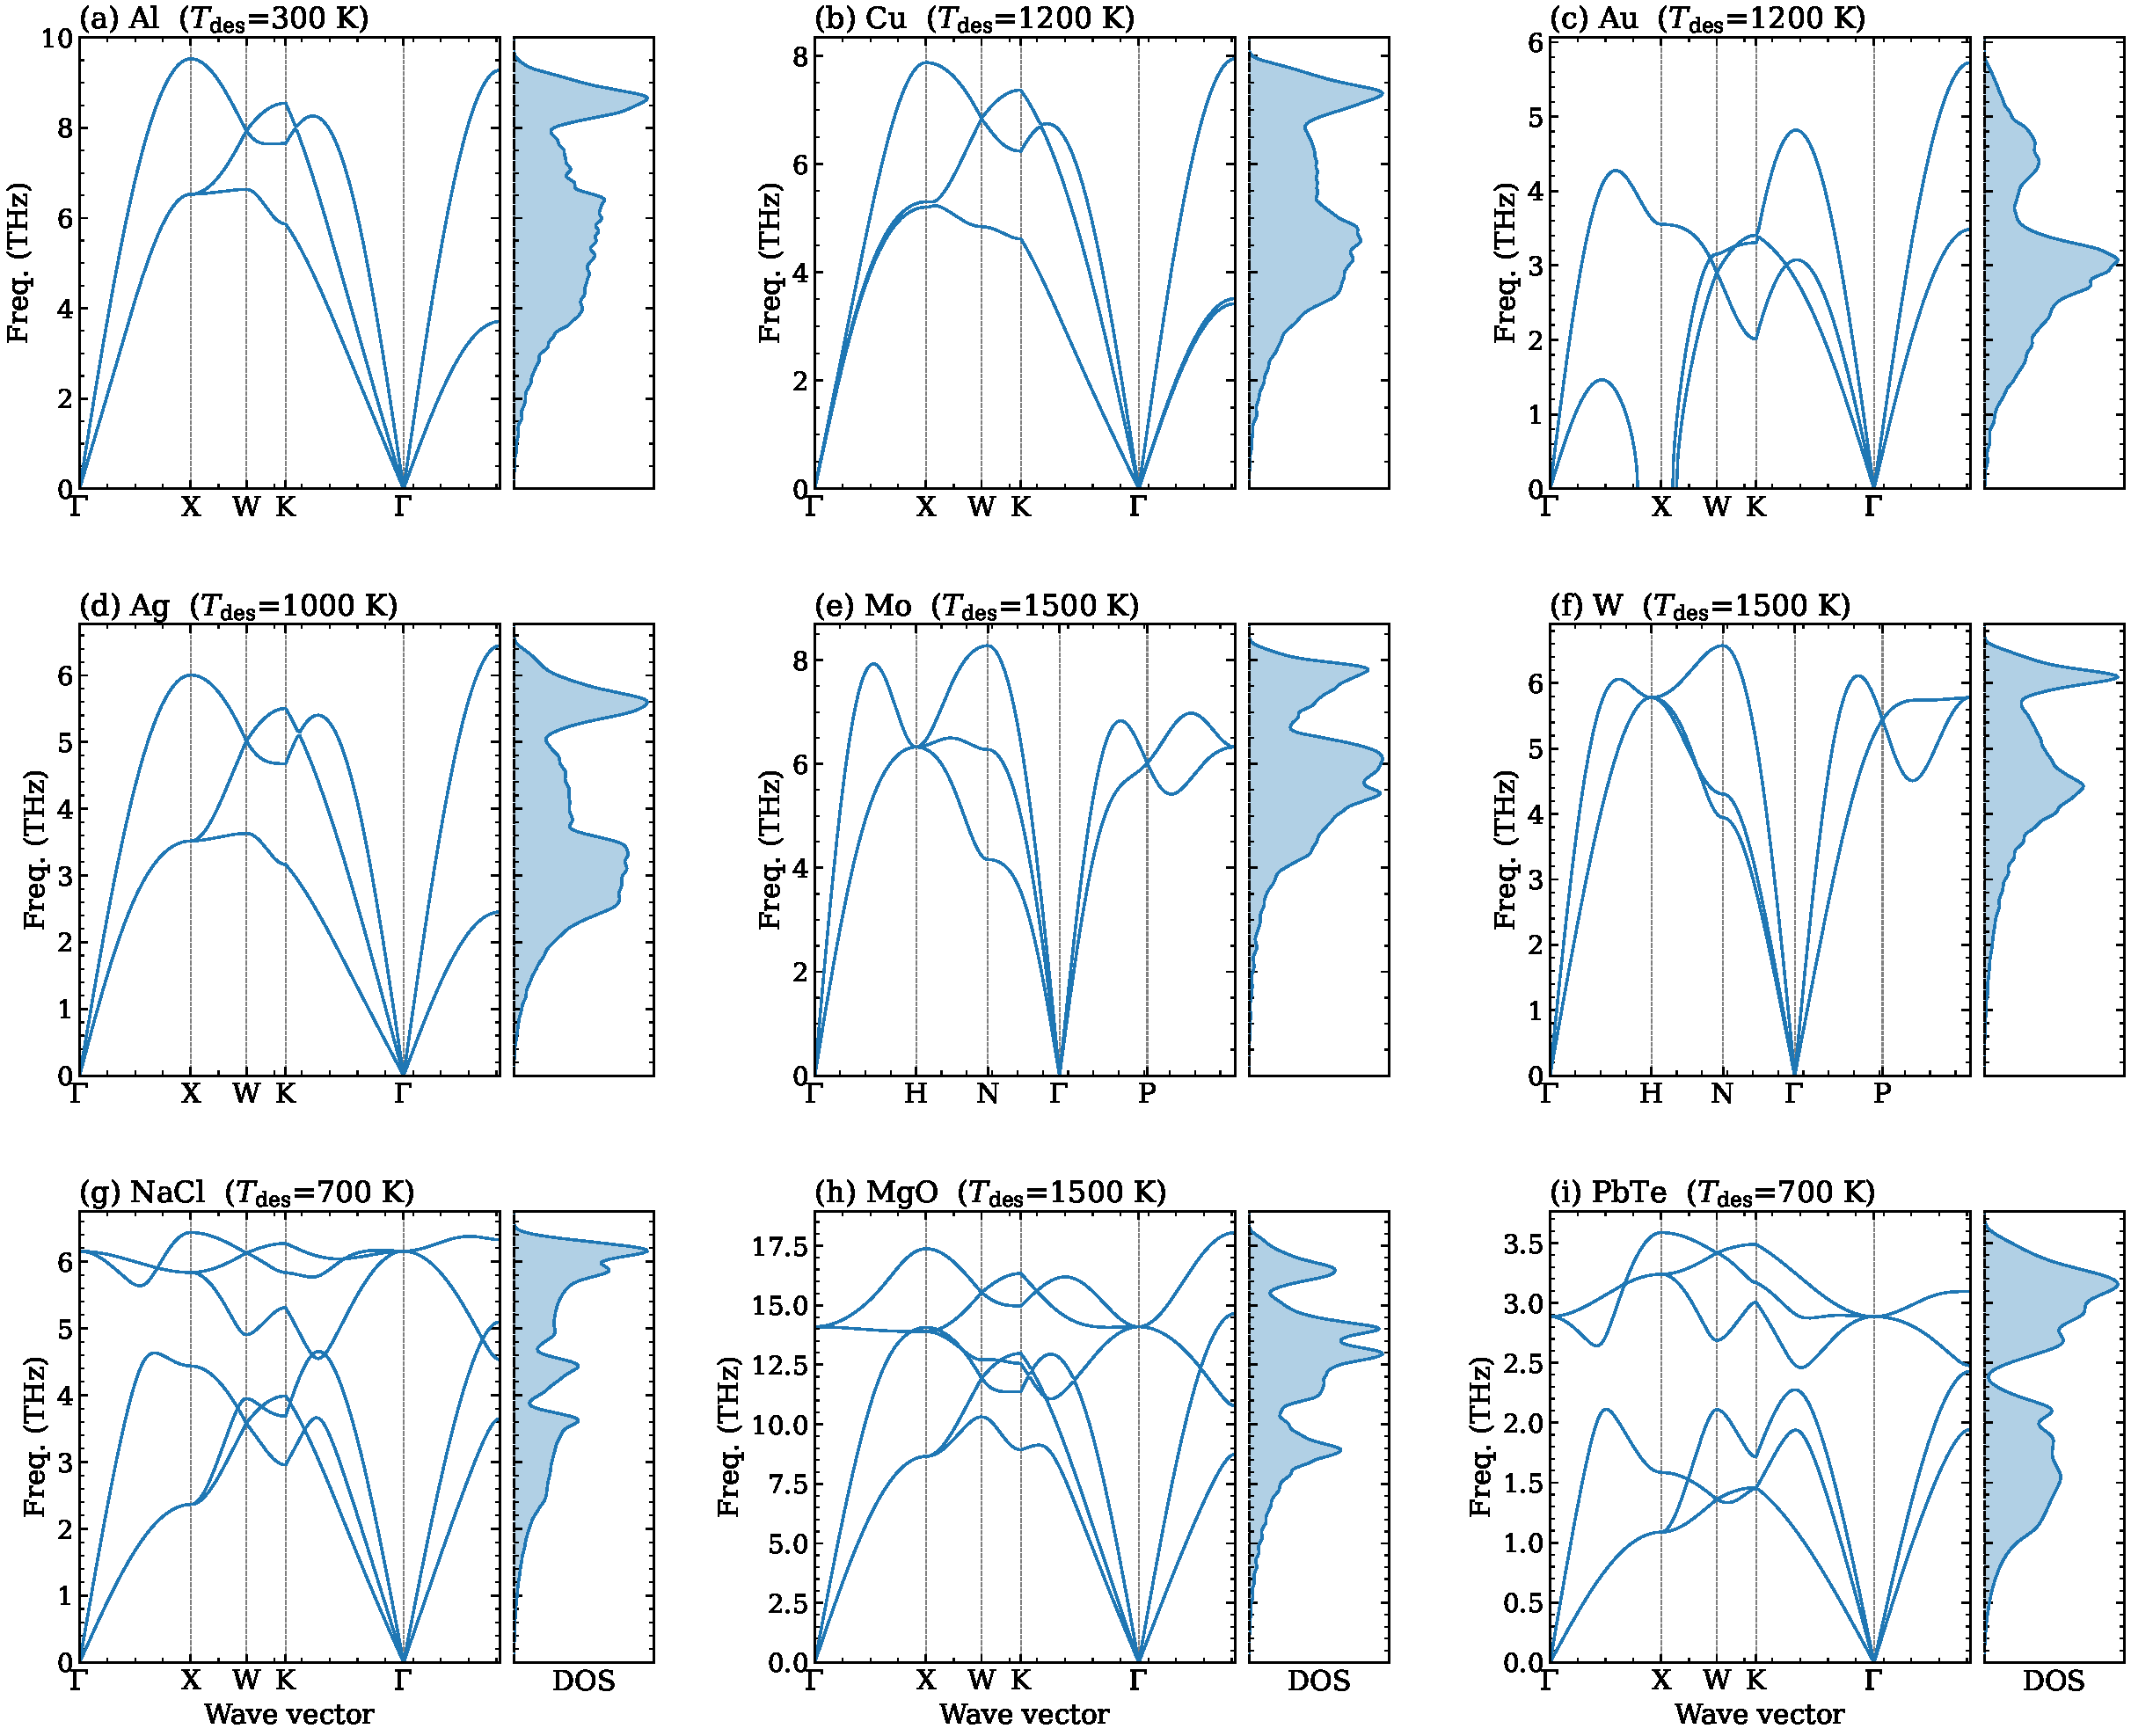
\includegraphics[width=\textwidth]{fig2_phonons_all.pdf}
\caption{Updated manuscript benchmark figure. Temperatures, stored paths,
omitted production-band NAC terms, and the Au instability are explicit; the
recoverable tabulated NaCl neutron data are shown in the separate LO--TO
figure.}
\end{figure}

\Question{5) The LO-TO splitting is missing for all three polar materials without a real clarification, which is relevant given that they represent a third of the entire benchmark set of materials. The calculation of the Born effective charge (BEC) tensor via DFPT is a standard capability of most DFT codes. Given that a DFPT calculation for the BEC tensor, using the primitive-cell, appears to be computationally cheaper than even one SOTC supercell evaluation, the reason why this is not included is not clear.}

\Answer{We agree. Primitive-cell QE~7.5 DFPT calculations are completed for
NaCl, MgO, and PbTe using PBE, 60/480~Ry wave-function/charge-density cutoffs,
an $8\times8\times8$ electronic mesh, a $10^{-10}$~Ry SCF threshold, and a
$10^{-14}$ DFPT threshold. They were evaluated at the corresponding production
lattice parameters 5.73, 4.26, and 6.51~\AA. The projected cubic
$(Z^*_{\rm cation},\varepsilon_\infty)$ pairs are
$(1.110915,2.470969)$, $(1.973385,3.167143)$, and
$(5.766700,28.826866)$, with equal and opposite anion charges.

Each tensor pair was applied through Phonopy's Wang formulation to an FC2 refit
of the actual selected production iteration. The selected iterations are 5, 4,
and 2, containing 3, 3, and 5 displaced snapshots, respectively; each
iteration's repeated equilibrium snapshot defines the reference force. The
resulting TO/LO/splitting values are 6.223/8.509/2.286~THz for NaCl,
14.097/22.144/8.047~THz for MgO, and 2.903/4.219/1.315~THz for PbTe. The no-NAC
conversion agrees with the native refit to better than $2\times10^{-6}$~THz RMSE.
The PbTe calculation is scalar-relativistic and does not test SOC sensitivity.

The independent conventional-FC2 NaCl control remains the stricter experimental
test: it gives 4.369~THz (TO), 7.264~THz (LO), and a 2.895~THz splitting versus
optical limits 4.917 and 8.034~THz, and it overlays 39 tabulated neutron points.
Figure~5 is now the quantitative production-model polar result. The older
production panels in Fig.~1 are explicitly labeled as no-NAC archival curves
and are not used as quantitative polar validation.

The production curves are reproducible selected-snapshot refits. Because the
selected in-memory FC2 objects were not serialized, we do not claim numerical
identity with the immutable no-NAC arrays in Fig.~1; instead, the refit
conversion is internally validated by reproducing its native no-NAC frequencies
to better than $2\times10^{-6}$~THz RMSE before applying NAC. This separates a
reproducible correction from an unsupported retroactive alteration of the
archived bands.}

\Change{Figures~4--5 and Sec.~IV.B (pp.~9--10) report same-volume DFPT
settings and apply the mass-normalized non-analytic correction to the
independent NaCl reference and selected-production refits for all three polar
compounds. Section~V.D (p.~13) distinguishes the immutable archival bands,
reproducible refits, experimental scope, and scalar-relativistic PbTe caveat.
Section~IV.B and the Conclusions report all three production-refit splittings.
Both new figures are reproduced below.}

\begin{figure}[htbp]
\centering
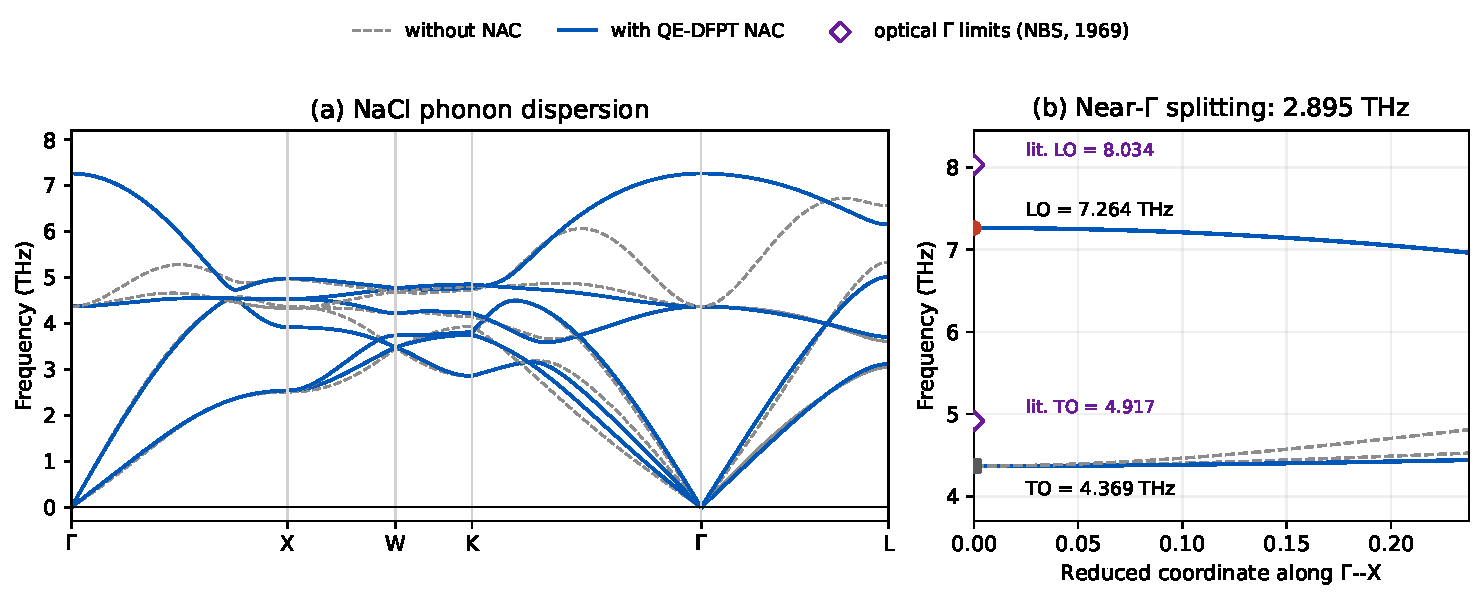
\includegraphics[width=0.95\textwidth]{fig_nacl_loto.pdf}
\caption{NaCl dispersion without and with the QE-DFPT non-analytic correction.
Red crosses are 39 tabulated 80~K neutron points along $\Gamma$--X and
$\Gamma$--L; purple diamonds are archival optical limits. The calculated TO
and LO limits are 4.369 and 7.264~THz, giving a 2.895~THz splitting.}
\end{figure}

\begin{figure}[htbp]
\centering
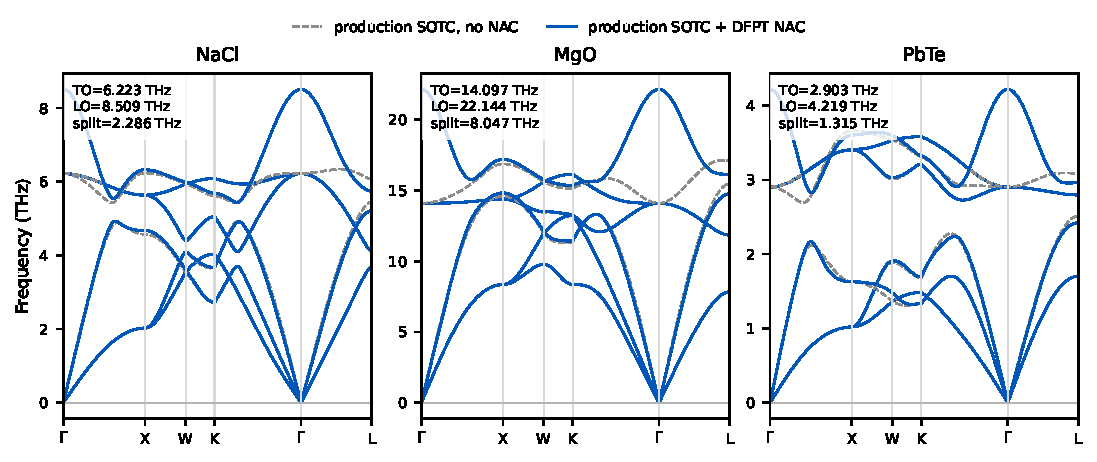
\includegraphics[width=\textwidth]{fig_polar_sotc_nac.pdf}
\caption{Selected-production FC2 snapshot refits without NAC (gray dashed) and
with same-volume QE-DFPT NAC (blue) for all three polar benchmarks. The
directional TO/LO/splitting values are printed in each panel.}
\end{figure}

\Question{6) The author states that ionic relaxation was not performed, employing experimental (non-relaxed) lattice parameters for all nine systems, and that all force evaluations are single-point calculations.

If the experimental equilibrium geometry does not coincide with the PBE energy minimum, which is essentially guaranteed, then the \textquotedblleft{}zero-displacement'' reference configuration used to build the SOTC displacement field is not a stationary point of the PBE potential energy surface, since nonzero residual forces on the atoms are expected even before any thermal displacement is applied.

This is important because Eq. (6) and (7) assume that $F=0$ at $u=0$. The author should demonstrate one of the following: i) demonstrate at least for one metal and one ionic compound, that the residual forces at the experimental geometry are negligible compared to the induced thermal displacement forces, ii) explain a residual-force substraction step (if this has been done, which is not currently described), or iii) perform a PBE-realxed geometry calculation showing that the thermodynamic results are compatible with the results employing the experimental geometry.}

\Answer{We implement option (ii) and have also quantified option (i).
All nine structures are ideal FCC, BCC, or rocksalt crystals with atoms on
symmetry-fixed Wyckoff sites. A mismatch between the experimental lattice
constant and the PBE minimum can therefore produce hydrostatic stress but does
not permit an internal atomic force in exact arithmetic. Numerical residuals
are nevertheless removed configuration by configuration using
$\Delta\mathbf F=\mathbf F(\mathbf u)-\mathbf F(\mathbf0)$ at the same cell
before drift projection and IFC fitting.

The archived independent campaigns directly verify the scale separation for
two metals and one ionic compound. Reference-force RMS values are
$1.67\times10^{-5}$, $2.45\times10^{-5}$, and
$8.34\times10^{-7}$~eV~\AA$^{-1}$ per Cartesian component for Al, W, and
NaCl, whereas induced-force RMS values are 0.395, 1.523, and
0.598~eV~\AA$^{-1}$. The induced/reference ratios are
$2.37\times10^4$, $6.22\times10^4$, and $7.17\times10^5$.
Thus residual atomic forces are negligible and explicitly subtracted in the
tested systems.

This does not imply volume relaxation: the corresponding stresses are 0.487,
$-0.761$, and 0.322~GPa. We therefore make no relaxed-volume or thermal-expansion
claim. The older primary summaries do not retain reference-force vectors, so
the numerical ratios are explicitly scoped to these archived controls; repeated
undisplaced calls in the primary inputs support only the force-call accounting.}

\Change{Equations~(6)--(7), Sec.~III.A (p.~4), and Appendix~D (p.~15)
now define reference-force subtraction before fitting. Section~III.A reports
the force ratios and distinguishes symmetry-forbidden internal forces from
finite cell stress; Sec.~V.D (p.~13) retains fixed-volume sensitivity as an
explicit limitation.}

\Question{Small details

i) Were the TDEP curves shown in Figs. 3--5 computed by the author with DFT settings matched to the SOTC-QE calculations, or are they taken from the literature? If from the literature, at what level of theory (functional, cell size, k-mesh)?}

\Answer{They were not supported by complete calculation-level provenance and have been removed. No TDEP curve remains. TDEP appears only in the related-method discussion, with the IFC rank and physical output stated.}

\Change{Figures and tables now compare SOTC only with experiment or with newly archived QE controls.}

\Question{ii) Phonopy is mentioned several times in the manuscript without introducing what it is. The author should not assume that all readers are familiar with this package.}

\Answer{Agreed. The first occurrence now identifies Phonopy as an open-source
finite-displacement and lattice-dynamics package and cites the primary
implementation paper; subsequent uses specify whether it generates the
conventional reference or applies the non-analytic correction.}

\Change{At first use, the manuscript now calls Phonopy a finite-displacement and lattice-dynamics software package and cites its primary implementation paper.}

\Question{iii) Code-specific implementation details about Quantum Espresso (QE) keywords and internal Python class names currently appear inside the theory section, for example, symmetrize bonds=True, SOTCQuasiHarmonic class, SOTCQuasiHarmonic(method=\textquotedblleft{}both''), \textquotedblleft{}degauss'' keyword, and so on. This can be useful for people already familiar with QE or with the Python script, but those details might be given separately in an appendix. The same applies for the pseudopotentials: in the computational details section, it is useful to know the pseudopotential details, but the actual file names can be relegated to an appendix.}

\Answer{Agreed. The main Theory section is implementation-independent. Scientific settings remain in Computational Details; file names, keyword spellings, data formats, scripts, and code flags are confined to the reproducibility appendix.}

\Change{The implementation material is now in the final appendix, ``Implementation, Reproducibility, and Data Availability.'' The main text contains no Python class name, file path, repository URL, JSON/NPZ/HDF5 reference, or literal QE keyword.}

\section*{Reviewer 3}

\Question{1. Structure and traceability of derivations. Several equations presented in the Theory section are, in fact, derived or more fully presented in the appendices, without clear indications in the main text. Beyond a single reference, the Theory section provides little indication of which results are original derivations versus material adapted from prior literature. The author should clearly indicate, at each equation, where derivations can be found and which results (if any) are drawn from existing work.}

\Answer{Agreed. Equation~(1) is identified as standard harmonic-lattice theory
and derived in Appendix~A. Equations~(2)--(3) are definitions/consequences of
Eq.~(1); Eq.~(4) is introduced here and linked to Appendix~C; Eq.~(5) is only a
numerical weight. Equation~(6) is now explicitly cited as the standard harmonic
force--displacement relation and points to Appendix~D for reference subtraction
and constrained assembly. Equations~(7)--(8) identify standard Tikhonov
regularization and dynamical-matrix construction; Eqs.~(9)--(12) are standard
harmonic thermodynamics.}

\Change{Section~II now identifies, at first use, whether each numbered equation is standard, a definition/consequence, or introduced in this work, and points to the corresponding appendix derivation. The text also distinguishes exact identities, numerical weights, modeling assumptions, and empirical results.}

\Question{2. Definition of the trace-averaged pair correlator. In Eq. (2), the trace-averaged scalar pair correlator $\bar{C}_2$ is defined such that $R$ becomes a scalar variable. It is unclear how this reduction is performed -- does it involve a spherical average over a shell of some finite width? This should be made explicit.}

\Answer{Equation~(2) defines the ideal crystallographic shell. The implemented
objective approximates it with finite 0.05~\AA\ radial bins and retains every
ordered basis/species-pair channel separately; it is not a continuum spherical
average or a full space-group-orbit construction. The bin width is now a
validated, explicit calculation input. The discarded anisotropic and
off-diagonal tensor information is stated as a limitation.}

\Change{Section~II.A, Sec.~III.B, Appendix~C, the archived calculation metadata,
and the implementation now state the 0.05~\AA\ shell-bin width consistently.}

\Question{3. Terminology: functional vs. multivariable function. The manuscript refers to $\mathcal{Q}$ (Eq. 4) as a \textquotedblleft{}functional.'' Strictly, a functional takes a function as its argument; here, $\mathbf{u}_i$ is a vector of $3n$ parameters, so $\mathcal{Q}$ is more accurately described as a multivariable function rather than a functional. This is a minor terminological point but should be corrected.}

\Answer{Agreed.}

\Change{Every applicable occurrence now says ``objective function'' or ``multivariable objective function.'' ``Functional'' remains only for a genuine free-energy functional.}

\Question{4. Exponential decay of the thermal two-point correlator (main concern). My principal concern is the claim -- made in the main text and repeated in Appendix B -- that the time-averaged thermal two-point correlator decays exponentially, attributed to a finite phonon lifetime arising from anharmonic effects. The Gr\"uneisen parameter appears in the associated formula, but no derivation, theoretical justification, or supporting reference is provided. Since the reduction in the number of required supercell displacements rests directly on this exponential-decay assumption, this gap is central to evaluating the method's validity, not a peripheral detail. A full derivation, or at minimum a clear literature justification, is needed.}

\Answer{We agree with the central criticism and have withdrawn the physical claim. A finite spectral lifetime does not establish universal exponential decay of an equal-time spatial correlator, particularly because acoustic modes can generate long-range or algebraic contributions. We removed the lifetime/Gr\"uneisen derivation, the purported thermal coherence length $\xi_T$, the $T^{-1}$ and $T^{-3}$ scaling laws, the 86\% norm claim, the 37-fold cost claim, and the representability theorem. The exponential $w(R;\xi_w)=e^{-R/\xi_w}$ is retained only as an optional positive numerical distance weight. It is not called a mean free path, and its length, cutoff, and supercell must be tested against mode-resolved frequency convergence. The small configuration counts are therefore no longer attributed to a proven exponential correlation bound.}

\Change{Section~II.B and Appendix~B now separate equal-time displacement correlations, dynamical phonon lifetime/mean free path, real-space IFC range, and numerical weighting. Appendices~E--G remove the rank, fixed-point, quadrature, and variational conclusions that depended on the unsupported decay argument. No theorem or universal configuration-scaling law remains in the abstract, main text, appendices, or Conclusions.}

\Question{5. Reliance on model dispersions rather than material-specific input. From Eq. (4), $\bar{C}_2$ enters as a required input, and Section Theory-E indicates that a model dispersion (Debye or Einstein) is used to compute it. This means little material-specific information enters the SOTC quality function, which raises the question of how the method can perform as well as claimed. It is difficult to assess the quality of the selected displacements without a baseline comparison. The author should include test cases comparing SOTC-selected displacements against random displacements to demonstrate a genuine advantage.}

\Answer{The production workflow uses the Debye model only to initialize the
first correlator; subsequent outer-loop targets use fitted material-specific
IFCs, masses, symmetry, and QE forces. We have now performed the requested
matched baseline at $N=1,2,4,8,16$ displaced-force calls. As detailed in our
response to Reviewer~1, comment~2, the cells, electronic settings, force
processing, FC2 priors, held-out set, and 251-point q paths are identical.
Twenty seeded canonical-Gaussian permutations are compared with three
pre-specified correlator-matched sequences initialized at $0.75T_D$, $T_D$,
and $1.25T_D$; every sequence and seed is shown in Fig.~3.

The pre-specified nominal comparison is the primary result. At 16 calls,
nominal SOTC gives 0.425, 0.223, and 0.548~THz for Al, W, and NaCl, versus
canonical medians 0.412, 0.207, and 0.564~THz. These differences are
$+3.2\%$, $+8.1\%$, and $-2.8\%$: nominal accuracy is comparable but not
uniformly better. Across all three pre-specified initializations the ranges are
0.404--0.574, 0.178--0.377, and 0.459--0.928~THz. The corresponding nominal
held-out-force errors are essentially the canonical medians. Accordingly, the
revised manuscript withdraws the universal-advantage claim and reports
comparability plus the complete sensitivity range.

The three sequences intentionally test the operational workflow, so Debye
target and optimizer seed vary together. They demonstrate practical
initialization sensitivity but do not isolate those two factors statistically.
Moreover, this test isolates initial displacement selection, not three complete
self-consistent outer-loop reruns. Both boundaries are stated in the figure
caption, Discussion, and Limitations.}

\Change{Figure~3 (p.~9) and Secs.~V.A--B (pp.~11--12) report all five
force-call counts, 20 canonical seeds, all three pre-specified initialization
sequences, displacement amplitudes, held-out-force errors, and pointwise
dispersion errors. Section~V.D (p.~13) states the coupled-initialization and
first-stage scope. The submitted superiority claim is replaced by the measured
nominal comparison and full sensitivity range.}

\begin{figure}[htbp]
\centering
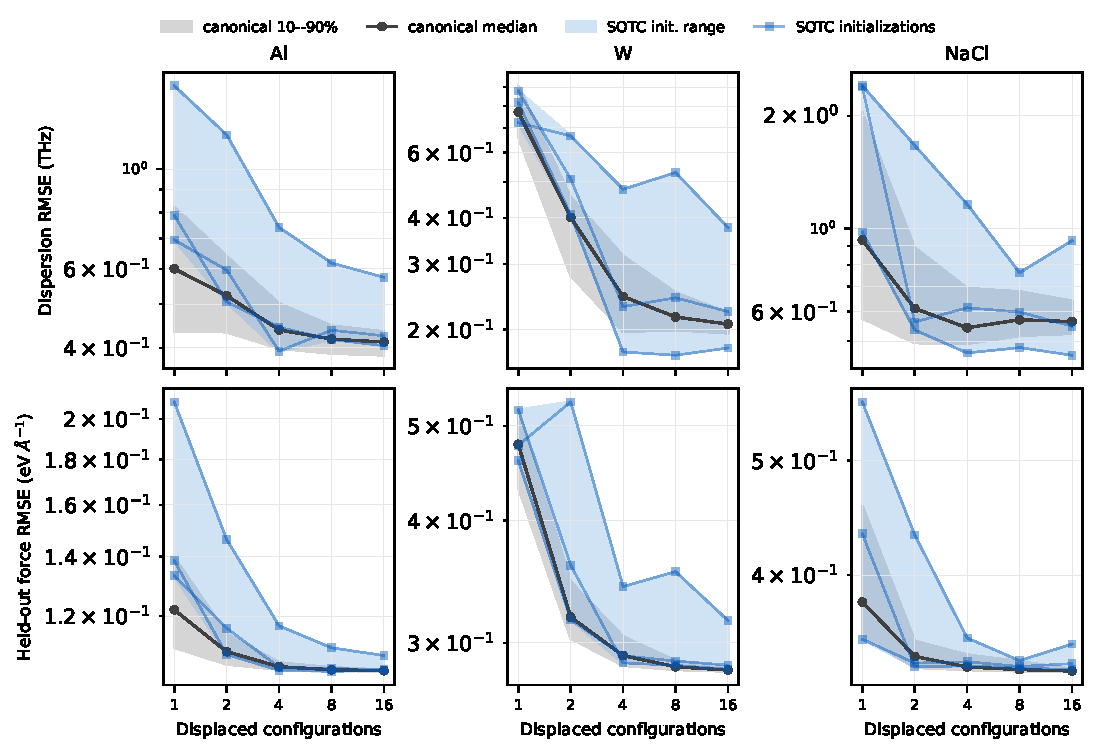
\includegraphics[width=\textwidth]{fig_matched_sampling.pdf}
\caption{New matched displacement-selection ablation. Dispersion RMSE (left)
and held-out force RMSE (right) are plotted against 1, 2, 4, 8, and 16
displaced-force calls for Al, W, and NaCl. Black bands show the 10--90\% range
over 20 canonical seeds; colored curves show three independently optimized
correlator-matched sequences initialized at $0.75T_D$, $T_D$, and $1.25T_D$.}
\end{figure}

\Question{6. Rank of the IFC matrix versus number of calculations. Each DFT calculation provides only a single direction in configuration space, and the author estimates the relevant IFC matrix rank to be of order 100. It is not clear how 2-5 calculations can yield a good approximation under these conditions. This may indicate that substantial physical prior knowledge (e.g., Debye temperature, acoustic sum rule) is already built into the method, which would help explain why aggregate quantities come out reasonably well despite the limited sampling. This should be discussed directly.}

\Answer{The revised paper no longer equates iteration count with DFT information or IFC identifiability. One $n$-atom force calculation supplies $3n$ scalar force equations, but it still samples one configuration-space direction and the stacked design can remain deficient. The primary runs use $N_{\rm ens}=1$--8 configurations per iteration and rely on the IFC cutoff, space-group/permutation reduction, central-force projection, acoustic sum rule, ridge regularization, trial-model initialization, and configuration stacking. Ridge can stabilize a deficient fit but cannot increase its algebraic rank or make it data-identifiable. The unsupported primary ranks were removed because the matrices and singular-value spectra were not archived.

The regression machinery was validated separately in 100-snapshot canonical campaigns for Al, NaCl, and W. Eighty snapshots train symmetry-, permutation-, translation-, and ASR-constrained FC2, FC2+FC3, and FC2+FC3+FC4 models; 20 inversion-paired snapshots are held out. The final parameter/rank values are 106/106, 48/48, and 126/126, with condition numbers 312.7, 36.9, and 269.4. Relative to matched conventional finite-displacement FC2, the final held-out force RMSE is reduced by 93.7\%, 72.3\%, and 87.5\%. This validates higher-order regression with a large ensemble; it does not establish FC3/FC4 recovery from the few-configuration SOTC workflow.

The new matched FC2 ablation supplies the complementary predictive check at
small $N$: held-out force error approaches a material-dependent plateau by
8--16 configurations even though that observation neither proves unique IFC
identification nor recovers an unavailable primary-run singular spectrum.
Accordingly, the revision reports rank only for saved matrices and predictive
error only on data excluded from fitting; it never infers one from the other.}

\Change{Table~I now reports material-specific iteration, ensemble, displaced-call, reference-call, and total-call counts rather than an ambiguous rank. Table~III and Appendix~E report rank only for saved designs. Sections~III.B, V.A--B, and V.D list the priors and distinguish scalar stopping-metric convergence, algebraic rank, predictive error, and cost. The new higher-order validation figure is reproduced below.}

\begin{figure}[htbp]
\centering
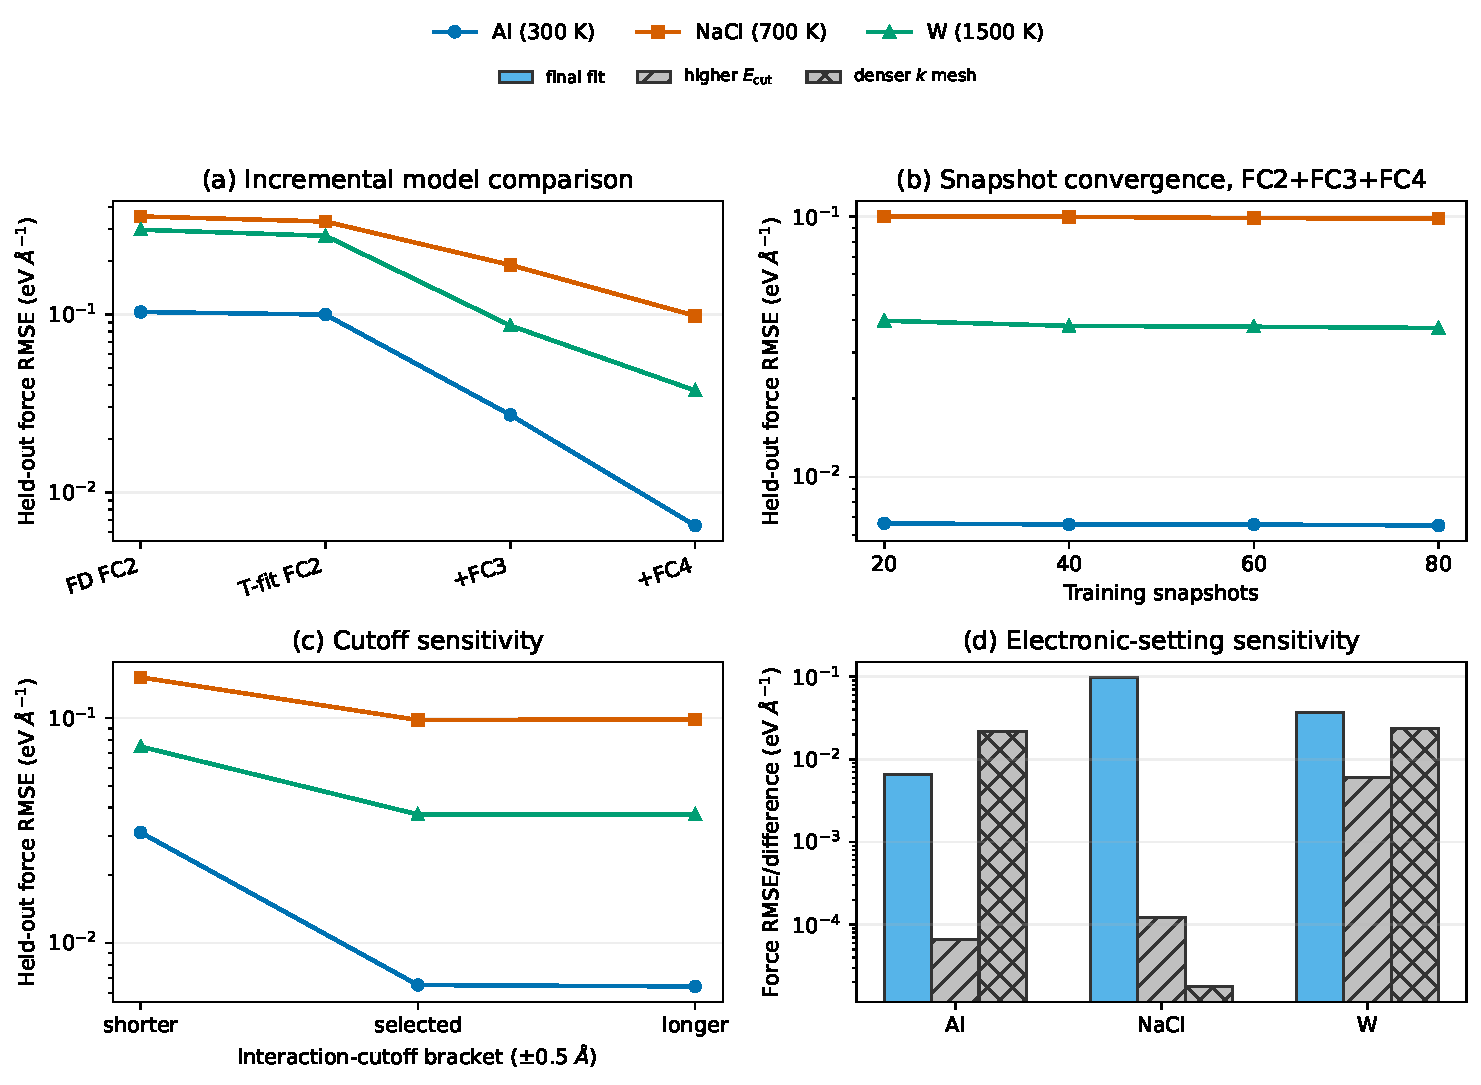
\includegraphics[width=0.95\textwidth]{fig_ifc34_diagnostics.pdf}
\caption{New manuscript figure: independent FC2/FC3/FC4 validation. The panels report held-out force RMSE, convergence with thermal-snapshot count, interaction-cutoff sensitivity, and electronic-setting force differences. This 100-snapshot campaign validates constrained higher-order regression, not higher-order recovery from the few-configuration SOTC design.}
\end{figure}

\Question{7. Comparison to AIMD, TDEP, and SSCHA (Discussion, subsection C). The comparison to these methods seems inappropriate: TDEP and SSCHA are specifically designed to capture anharmonic effects, whereas the present results are obtained within the harmonic approximation (with thermal lattice expansion treated quasi-harmonically, as far as I can tell). The method proposed here does not appear to address the same physical problem as TDEP and SSCHA, and the comparison should be reframed or qualified accordingly.}

\Answer{Agreed. SOTC is described as deterministic configuration design plus
effective-FC2 fitting. TDEP fits effective IFCs to supplied ensemble data; SCHA
is the variational effective-harmonic level and SSCHA its stochastic
implementation. The manuscript explicitly acknowledges that converged sTDEP and
sSCHA can reach the same effective-harmonic stationary solution and free energy
under consistent conditions. No comparison of explicit anharmonic free
energies, lifetimes, transport, or renormalized spectra is claimed.}

\Change{The abstract, Introduction, Sec.~V.C, Limitations, and Conclusions now separate physical level and IFC rank explicitly.}

\Question{8. Reliance on aggregate quantities tied to the phonon density of states. Many of the reported physical quantities depend primarily on the phonon density of states $g(\omega)$, which tends to obscure details of the underlying dispersion through integration -- meaning that a mediocre $g(\omega)$ can still yield reasonable aggregate properties. To convincingly demonstrate the superiority of the SOTC approach, the author should provide direct comparisons of the phonon dispersion itself -- for example, showing convergence of the dispersion as a function of the number of displacements included -- compared against fully converged DFT results. I also note that the Au phonon dispersion in Fig. 2 shows instabilities, which points to a problem with the method and should be addressed explicitly.}

\Answer{We agree. The new matched calculation compares pointwise sorted-mode
dispersion at $N=1,2,4,8,16$ displaced-force calls against the same-cell
conventional QE/Phonopy FC2 target. That target uses 0.01~\AA central finite
displacements, identical electronic settings, and the same 251-point path. It
is the deterministic harmonic reference for the fixed periodic cell, which is
the appropriate target for isolating displacement-selection error. We do not
mislabel it as an infinite-supercell or complete-basis thermodynamic limit.

The canonical median RMSE sequences are
0.600/0.522/0.438/0.418/0.412~THz for Al,
0.772/0.401/0.245/0.216/0.207~THz for W, and
0.933/0.611/0.543/0.570/0.564~THz for NaCl. The nominal-$T_D$
correlator-matched sequences are 0.696/0.596/0.393/0.438/0.425,
0.879/0.509/0.230/0.243/0.223, and
2.390/0.563/0.614/0.598/0.548~THz. Figure~3 additionally shows the canonical
10--90\% ranges, both $\pm25\%$ initialization sequences, and held-out force
RMSE. These direct branch-resolved curves, not DOS-integrated observables, are
the basis of the sampling conclusion. Their small non-monotonic changes at
large $N$ are reported rather than smoothed or described as strict convergence.

The Au audit finds a minimum frequency of $-1.066$~THz at X, reduced q point
$(0.5,0,0.5)$, on the lowest branch. Frequencies below $-0.05$~THz account for
45 of 753 plotted branch/q-point values (5.98\%) over indices 40--63 around X.
The mesh instability fraction increases from 0.39\% at iteration 1 to 15.6\%
at iteration 2. The archived data cannot isolate cell, cutoff, regularization,
projection, electronic, or volume effects. Au is therefore excluded from the
stable-dispersion evidence, and no aggregate Au observable is used to imply a
validated dispersion.}

\Change{The new control gives pointwise sorted-mode conventional-FC2 errors
and matched error-versus-count convergence for 20 canonical seeds and all three
correlator-matched initializations. The cells, electronic settings, force
processing, fitting choices, held-out set, q paths, and displaced-force counts
are identical. The test is explicitly scoped to first-stage selection and
three materials rather than claimed as universal outer-loop convergence. The
Au instability is quantified and scoped, and DOS-integrated agreement is not
presented as proof of accurate dispersion.}

\end{document}
